%!TEX root = main.tex
\chapter[Implementaci\'on]{PRVO y $\mu$Java++}
\label{cap:implementation}

\section{$\mu$Java++}

La herramienta \emph{$\mu$Java} \cite{bibliography.mutation.tools.muJavaMaOK05} funciona traduciendo c\'odigo fuente \emph{Java} a un \emph{AST}, una estructura de \'arbol que representa el c\'odigo original como nodos, y recorriendo el mismo mediante un patr\'on \emph{visitor}. Cada operador sobreescribe m\'etodos particulares de visita para los nodos objetivo, el operador \emph{ROR}, por ejemplo, solo tiene por objetivo a expresiones binarias (en cuanto al tipo de nodos) y particularmente a aquellas que utilicen un operador relacional. En la Figura~\ref{figures.examples.rorMutation} se ve una parte de un \emph{AST} correspondiente a la sentencia \lstinline|x = y < 0|, \emph{ROR} al visitar el nodo \emph{BinExpr} con el operador \emph{<}, va a generar varias mutaciones, entre otras, el nodo mutado \emph{BinExpr[>]} que corresponde al cambio de el operador \emph{<} por \emph{>}, mientras mantiene los subnodos de \emph{BinExpr} sin modificaciones.

\begin{figure}
	\centering
	\begin{tikzpicture}%
	[state/.style ={ellipse, draw, minimum width = 0.7 cm},
	point/.style = {circle, draw, inner sep=0.04cm,fill,node contents={}},
	el/.style = {inner sep=2pt, align=left, sloped}]
	\node[state,rectangle] (asg) {$Assignment$};
	\node[state,rectangle] (varx) [below=of asg] {$Var[x]$};
	\node[state,rectangle] (bexpr) [right=of varx] {$BinExpr[<]$};
	\node[state,rectangle] (vary) [below=of bexpr] {$Var[y]$};
	\node[state,rectangle] (lit) [right=of vary] {$Lit[0]$};
	
	\path (asg) edge (varx);
	\path (asg) edge (bexpr);
	\path (bexpr) edge (vary);
	\path (bexpr) edge (lit);
	
	\node[draw=blue,dotted,fit=(bexpr) (vary) (lit), inner sep=0.2cm] (binaryO) {};
	
	\node[state, rectangle] (bexprM) [right=of binaryO] {$BinExpr[>]$};
	
	\path[->] (binaryO) edge[bend left=20] node[above] {ROR} (bexprM);
	\path (bexprM) edge[bend right=20] (vary);
	\path (bexprM) edge[bend right=20] (lit);
	
	\end{tikzpicture}
	\caption[El operador \emph{ROR} sobre un \emph{AST}]{Ejemplo del operador \emph{ROR} en funcionamiento}
	\label{figures.examples.rorMutation}
\end{figure}

Una de las primeras tareas para poder desarrollar \emph{PRVO}, fue la reimplementaci\'on de esta herramienta. Hay dos herramientas involucradas, una es \emph{OJ}, anteriormente conocida como \emph{OpenJava}, que permite la transformaci\'on de c\'odigo fuente \emph{Java} en un \emph{AST}, as\'i como ofrecer clases para el recorrido y modificaci\'on de el mismo. \'Esta es la base que utiliza \emph{$\mu$Java}, y actualmente \emph{$\mu$Java++}. Ambas herramientas fueron altamente modificadas, con \emph{$\mu$Java} siendo pr\'acticamente reescrita por completo. Las razones para realizar dicha tarea tiene que ver con una serie de requerimientos que definimos a continuaci\'on:

\subsection{Representaci\'on}

Originalmente, las mutaciones no estaban representadas en \emph{$mu$Java}, los mutantes se generaban directamente, muchas veces como una responsabilidad del operador. Al dise\~nar \emph{PRVO}, observamos que era muy f\'acil generar mutaciones repetidas, tomemos por ejemplo la expresi\'on \lstinline|a.b.c|, es posible generar \lstinline|a.c| eliminando la subexpresi\'on del medio, pero tambi\'en es posible al reemplazar las dos primeras por \lstinline|a|. Al mismo tiempo, la variable especial \lstinline|this|, permite que para todo campo de una clase, haya dos formas de referirse al mismo, una mediante el uso de \lstinline|this|, y otra obviando el mismo. Por otro lado, \emph{PRVO} estaba siendo muy utilizado en el desarrollo de \emph{Stryker}, herramienta de reparaci\'on autom\'atica, la cual se describe en la secci\'on \ref{sec:repair.striker}. La necesidad de contar con cierta informaci\'on sobre las mutaciones para permitir ordenar e incluso ignorar algunas durante la b\'usqueda de un potencial arreglo, nos llev\'o a definir una representaci\'on para las mutaciones generadas mediante ternas \texttt{(original, mutante, operador)} en donde los dos primeros elementos representan, respectivamente, el nodo original y mutado del \emph{AST} y el tercero denota el operador utilizado. \'Estas se almacenan durante la generaci\'on de mutaciones hasta que se decida generar los mutantes, esto permite, entre otras cosas, analizar y evitar mutaciones repetidas.

\subsection{Anotaciones y control de generaciones}

Las herramientas de mutaci\'on, suelen no contar con un control sobre que partes de c\'odigo se van a mutar, o \'este es muy grueso, por ejemplo al permitir definir clases y m\'etodos a mutar. Debido nuevamente a los comienzos orientados a reparaci\'on de \emph{PRVO}, necesit\'abamos un control m\'as fino sobre donde se aplicar\'ian las mutaciones. Lo que nos llev\'o, adem\'as de permitir definir que m\'etodos se permiten mutar, a utilizar comentarios \lstinline|//mutGenLimit K| luego de una sentencia para permitir que solo aquellas que tengan estas anotaciones y el \emph{K} sea mayor a 0, sean mutadas.

A su vez, las anotaciones utilizadas son escritas en el mutante con el \emph{K} asociado disminu\'ido en 1. Esto permite, en casos como reparaci\'on o generaci\'on de mutantes compuestos (aquellos con m\'as de una mutaci\'on aplicada), controlar las generaciones m\'aximas por sentencia.

\subsection{Estandarizaci\'on de componentes}

La versi\'on original de la herramienta ten\'ia implementaci\'ones muy diferentes por operador, algunos escrib\'ian directamente cada mutante (sin tener una representaci\'on para las mutaciones aplicadas), esto hac\'ia que desarrollar nuevos operadores fuera una tarea compleja, nuestra versi\'on permite desarrollar nuevos operadores con relativa facilidad. Durante el desarrollo de \emph{PRVO}, tuvimos en cuenta que en el futuro podr\'iamos querer implementar nuevos operadores, y funcionalidades, lo que nos llev\'o a re-dise\~nar grandes partes de la herramienta. Gracias a esto, pudimos utilizar a \emph{$mu$Java++} para desarrollar otro operador de mutaci\'on, \emph{BEE} \cite{bibliography.mutation.operators.beeBridaS17}, centrado en generar mutaciones para fortalecer y debilitar expresiones condicionales de una manera m\'as fina que operadores existentes, a su vez, pudimos implementar funcionalidades de an\'alisis descriptas a continuaci\'on.

\subsection{Evaluaci\'on}

Mutation testing consiste en generar mutantes y evaluar cuantos son detectados por el conjunto de tests en evaluaci\'on. En la secci\'on \ref{sec:preliminares.mutation.opevaluation} se mencionan varias caracter\'isticas que afectan a este criterio, en particular dificultad de detecci\'on y redundancia de mutantes. Nuestra versi\'on de \emph{$\mu$Java} provee ciertas mejoras en el an\'alisis con respecto a estas propiedades, como ofrecer dos valores de \emph{mutation score}, uno en donde se consideran los mutantes que no compilaron y otro donde no se los considera. Si bien, una evaluaci\'on inicial y muy b\'asica de dificultad de detecci\'on, \emph{$mu$Java++} ofrece un an\'alisis de ``dureza'' de los mutantes, al analizar, cuantos tests fue capaz de sobrevivir cada mutante. Con respecto a redundancia, un an\'alisis m\'as complejo que ofrece nuestra herramienta, es \emph{dynamic mutant subsumption}, en donde se genera un grafo de subsunci\'on de mutantes para la test suite particular, permitiendo evaluar que mutantes fueron redundantes y cuales son indispensables. Finalmente, para lidiar con la explosi\'on de mutantes que se puede dar, y c\'omo el rendimiento es afectado por eso, se implementaron la capacidad de frenar la ejecuci\'on de los tests para un mutante cuando \'este es detectado (perdiendo ciertos an\'alisis que requieren datos completos de la ejecuci\'on de los tests), y el an\'alisis en paralelo de mutantes para acelerar el proceso.

\section{PRVO}
\label{sec:implementation.prvo}

La definici\'on general de \emph{PRVO}, dada en \ref{sec:prvo.prvo}, no es efectiva en la pr\'actica, desde ya por que permite entre otras cosas, infinitas mutaciones. Si bien mencionamos, e incluso presentamos a \emph{PRVO} como un meta-operador altamente configurable, es necesario establecer algunas restricciones b\'asicas, ya que mientras m\'as flexible es un operador, m\'as compleja es su implementaci\'on. Por esta raz\'on, es que decidimos fijar ciertas restricciones iniciales, basadas en la evoluci\'on de \emph{PRVO} durante su desarrollo, tanto en su uso en reparaci\'on, como en mutation testing.

Inicialmente \emph{PRVO} comienza como una necesidad en reparaci\'on autom\'atica de programas. Utilizando la herramienta \emph{Stryker}, \emph{PRVO} provee el potencial de reparar ciertos defectos no reparables por herramientas tradicionales de reparaci\'on autom\'atica. Como un problema que se menciona en \ref{cap:repair}, la explosi\'on de candidatos a reparaci\'on es uno de los principales obst\'aculos que se deben afrontar en el dise\~no de herramientas de reparaci\'on. Por esto, \emph{PRVO} comienza con una serie de restricciones sobre el tama\~no de las expresiones mutadas, la diferencia entre el tama\~no original y final de una expresi\'on no puede superar a \texttt{1}. Estas restricciones llevan a una definici\'on m\'as acotada, provista en la Figura~\ref{figures.definitions.prvo.impl_def}, que la original provista en la Figura~\ref{figures.definitions.prvo.simple_def}. Es necesario realizar una aclaraci\'on sobre el valor \texttt{null}, es posible reducir una expresi\'on a este valor y es posible reemplazar a \texttt{null}, pero no es posible extender a este valor.

\begin{figure}[H]
	\begin{enumerate}[leftmargin=.75cm,align=left]
		\item [Inserci\'on] Si $A\::\:Expr(D \rightarrow T)$ en el contexto $\rho$, y el tama\~no de $A$ es $k$, entonces $\forall b \in \rho \:\cdot\:  \forall e \in interleave(b, A)\:\cdot\: e\::\: Expr(D \rightarrow T) \rightarrow e\in\:PRVO(A, \rho)$ y el tama\~no de las expresiones generadas es de $k+1$
		\item [Sustituci\'on] Si $A\::\:Expr(D \rightarrow T)$ en el contexto $\rho$, y el tama\~no de $A$ es $k$, entonces $\forall a \in A \:\cdot\: \forall b \in \rho \:\cdot\: a\::\:D_1 \rightarrow T_1 \wedge b\::\:D_1 \rightarrow T_1 \rightarrow A[a := b] \in\:PRVO(A, \rho)$ y el tama\~no de las expresiones generadas es de $k$
		\item[Eliminaci\'on] Si $A\::\:Expr(D \rightarrow T)$ en el contexto $\rho$, y el tama\~no de $A$ es $k$, entonces $\forall a \in A \:\cdot\: e = remove(a,A) \wedge e\::\:Expr(D \rightarrow T) \rightarrow e\in\:PRVO(A, \rho)$ y el tama\~no de las expresiones generadas es de $k-1$
		\item[Sustituci\'on 1x2] Si $A\::\:Expr(D \rightarrow T)$ en el contexto $\rho$, y el tama\~no de $A$ es $k$, entonces $\forall a \in A \:\cdot\: \forall b,c \in\rho \:\cdot\: a\::\:D_1 \rightarrow T_1 \wedge \rho\vdash[b,c]\::\:Expr(D_1 \rightarrow T_1) \rightarrow A[[a] := [b,c]] \in\:PRVO(A, \rho)$ y el tama\~no de las expresiones generadas es de $k+1$
		\item[Sustituci\'on 2x1] Si $A\::\:Expr(D \rightarrow T)$ en el contexto $\rho$, y el tama\~no de $A$ es $k$, entonces $\forall a,b \in A \:\cdot\: [a,b]\::\:Expr(D_1 \rightarrow T_1) \rightarrow \forall c \in \rho \:\cdot\: c \::\: D_1 \rightarrow T_1 \rightarrow A[[a,b] := c] \in\:PRVO(A, \rho)$ y el tama\~no de las expresiones generadas es de $k-1$
	\end{enumerate}
	\caption{Definici\'on base de la implementaci\'on de \emph{PRVO}}
	\label{figures.definitions.prvo.impl_def}
\end{figure}


\subsection{Configuraci\'on de PRVO}

Con el tiempo la cantidad de comportamientos o restricciones configurables en \emph{PRVO} fue aumentando. En esta secci\'on solo mencionaremos un conjunto de \'estas, ya que varias fueron implementadas para casos muy particulares.

\subsubsection{Restricciones de tama\~no}
\label{sec:implementation.prvo.restrictions.size}

La definici\'on de \emph{PRVO} provista en la Figura~\ref{figures.definitions.prvo.impl_def} define 5 mecanismos independientes mediante los cuales se generan las mutaciones. A continuaci\'on se proveen descripciones m\'as informales de los mismos:

\begin{enumerate}[leftmargin=.75cm,align=left]
	\item[\textbf{Reemplazar un elemento (R)}] Ciertas mutaciones de \emph{PRVO} solo modifican elementos unitarios (expresiones de tama\~no 0) en una expresi\'on, reemplaz\'andolos por otros de tama\~no 0.
	
	\item[\textbf{A\~nadir un elemento (A)}] Una expresi\'on puede incrementarse por 1 su tama\~no, al insertar un elemento tanto al principio, al final, o intercalarlo en su interior.
	
	\item[\textbf{Eliminar un elemento (D)}] En una expresi\'on de navegaci\'on, se puede eliminar un elemento, ya sea al principio, final, o en el resto de la expresi\'on. No es posible eliminar un elemento en una expresi\'on que no hace uso del operador de navegaci\'on (tiene tama\~no 0), ya que no hay ninguna subexpresi\'on para remover.
	
	\item[\textbf{Intercambiar dos elementos por uno (2x1)}] Dada una expresi\'on de navegaci\'on, dos elementos contiguos, es decir, una subexpresi\'on de navegaci\'on de tama\~no 1, puede ser reemplazada por un \'unico elemento, es decir, una expresi\'on de tama\~no 0.
	
	\item[\textbf{Intercambiar un elemento por dos (1x2)}] En una expresi\'on, un elemento de la misma puede ser reemplazado por dos elementos contiguos, es decir, una expresi\'on de navegaci\'on de tama\~no 1.
\end{enumerate}

En el ejemplo siguiente pueden verse algunas de las distintas mutaciones que corresponden a las restricciones anteriores, en algunos casos el mismo mutante puede ser logrado por distintas mutaciones:
\begin{lstlisting}[mathescape=true,language=Java,basicstyle={}]
  current = current.next; //original
  $\delta$current = header; //2x1
  $\delta$current = current; //2x1 o D 
  $\delta$current = current.next.next; //1x2 o A
  $\delta$current = header.previous.next; //1x2 o A
  previous = current; //original
  $\delta$previous = header; //R
  $\delta$previous = null; //R
  $\delta$previous = current.next; //1x2 o A
  $\delta$previous = header.next; //1x2
\end{lstlisting}

En las Figuras \ref{figures.code.prvoMethods.sameLength}, \ref{figures.code.prvoMethods.increaseLength}, \ref{figures.code.prvoMethods.decreaseLength}, \ref{figures.code.prvoMethods.twoByOne}, y \ref{figures.code.prvoMethods.oneByTwo}, se muestran versiones muy simplificadas de los m\'etodos de \emph{PRVO} para generar mutaciones (reemplazo por literales, por ejemplo, no se muestra). M\'etodos auxiliares utilizados por \'estos incluyen a:

\begin{enumerate}[leftmargin=.75cm,align=left]
	\item[\textbf{generateMutant(Expression, Expression) : void}]\mbox{}\\ Este m\'etodo reemplaza la expresi\'on original (primer par\'ametro) por la expresi\'on mutada (segundo argumento) en el AST (Abstract Syntax Tree) relacionado al programa para el cual se est\'an generando mutantes.
	
	\item[\textbf{append(Expression...) : void}]\mbox{}\\ Este m\'etodo toma una secuencia de expresiones de navegaci\'on y las une mediante el operador de navegaci\'on (\emph{punto}), los argumentos nulos son ignorados.
	
	\item[\textbf{isReachable(Expression, Expression) : boolean}]\mbox{}\\ Este m\'etodo verifica si la primera expresi\'on de navegaci\'on es alcanzable desde la segunda, es decir, si el primer elemento de la primera expresi\'on de navegaci\'on representa un miembro del tipo del \'ultimo elemento de la segunda. Por ejemplo \lstinline{next.value} es alcanzable desde \lstinline{this.header} en una lista (ver Figura~\ref{figures.examples.navigationExprGraph}).
	
	\item[\textbf{elements(Expression) : [Expression]}]\mbox{}\\ Retorna una lista de todos los elementos que conforman una expresi\'on de navegaci\'on. Por ejemplo, la expresi\'on \lstinline{current.next.value} retornar\'ia una lista con \lstinline{current}, \lstinline{next}, y \lstinline{value}.
	
	\item[\textbf{getType(Expression) : Type}]\mbox{}\\ Este m\'etodo retorna el tipo asociado al \'ultimo elemento de una expresi\'on de navegaci\'on. Por ejemplo, para la expresi\'on \lstinline{current.next} retornar\'ia \lstinline{Node} (ver Figura~\ref{figures.examples.navigationExprGraph}).
	
	\item[\textbf{compatibleTypes(Type, Type) : boolean}]\mbox{}\\ Este m\'etodo verifica si el primer tipo es compatible con el segundo. La compatibilidad ser\'a verificada de acuerdo a la configuraci\'on de \emph{PRVO}, si el chequeo de tipos es relajada, entonces se verifica si el primer tipo es asignable al segundo; si por el contrario se est\'a utilizando un chequeo de tipos estricto, entonces solo son compatibles los tipos iguales.
	
	\item[\textbf{fieldsAndMethodsFrom(Expression) : [Expression]}]\mbox{}\\ Retorna todos los miembros accesibles desde el \'ultimo elemento de una expresi\'on de navegaci\'on (no nula).
	
	\item[\textbf{reachableVarsFieldsAndMethods() : [Expression]}]\mbox{}\\ Retorna todas las variables, campos y m\'etodos que son alcanzables desde el punto actual.
	
	\item[\textbf{nextExpression(Expression) : Expression}]\mbox{}\\ Dada una expresi\'on de navegaci\'on retorna \emph{null} si \'esta no est\'a conectada mediante el operador de navegaci\'on a otra, o retorna la expresi\'on de navegaci\'on a la cual est\'a conectada mediante el operador de navegaci\'on en caso contrario. Cabe destacar que si bien el m\'etodo \lstinline{elements(Expression)} retorna elementos desconectados, \'estos tienen asociados a que expresiones de navegaci\'on estaban previamente conectados.
	
	\item[\textbf{previousExpression(Expression) : Expression}]\mbox{}\\ Equivalente a \lstinline{nextExpression(Expression)} pero retornando la expresi\'on de navegaci\'on a la cual \'esta estaba conectada (o \lstinline{null} si no lo estaba).
	
	\item[\textbf{lastExpressionFrom(Expression) : Expression}]\mbox{}\\ Retorna el \'ultimo elemento en una expresi\'on de navegaci\'on, el cual es la expresi\'on original si \'esta es de tama\~no $0$, o el \'ultimo miembro en caso contrario. Por ejemplo \lstinline{lastExpressionFrom(current.next.value)} retornar\'ia \lstinline{value}, mientras que \lstinline{lastExpressionFrom(current)} retornar\'ia \lstinline{current}.
\end{enumerate}

\begin{figure}
	\lstinputlisting[basicstyle=\small, language=Java, tabsize=3]{results/draft/PRVO_sameLength.java}
	\caption[Funciones \emph{PRVO}, \emph{\#sameLength}]{M\'etodo de generaci\'on de mutantes de \emph{PRVO} para generar expresiones donde el tama\~no de la misma se mantiene.}
	\label{figures.code.prvoMethods.sameLength}
\end{figure}

\begin{figure}
	\lstinputlisting[basicstyle=\small, language=Java, tabsize=3]{results/draft/PRVO_increaseLength.java}
	\caption[Funciones \emph{PRVO}, \emph{\#increaseLength}]{M\'etodo de generaci\'on de mutantes de \emph{PRVO} para generar expresiones donde el tama\~no de la misma se incrementa a\~nadiendo un nuevo elemento a la expresi\'on.}
	\label{figures.code.prvoMethods.increaseLength}
\end{figure}

\begin{figure}
	\lstinputlisting[basicstyle=\small, language=Java, tabsize=3]{results/draft/PRVO_decreaseLength.java}
	\caption[Funciones \emph{PRVO}, \emph{\#decreaseLength}]{M\'etodo de generaci\'on de mutantes de \emph{PRVO} para generar expresiones donde el tama\~no de la misma se decrementa eliminando un elemento de la expresi\'on.}
	\label{figures.code.prvoMethods.decreaseLength}
\end{figure}

\begin{figure}
	\lstinputlisting[basicstyle=\small, language=Java, tabsize=3]{results/draft/PRVO_twoByOne.java}
	\caption[Funciones \emph{PRVO}, \emph{\#twoByOne}]{M\'etodo de generaci\'on de mutantes de \emph{PRVO} para generar expresiones donde el tama\~no de la misma se decrementa reemplazando dos elementos de una expressi\'on por uno.}
	\label{figures.code.prvoMethods.twoByOne}
\end{figure}

\begin{figure}
	\lstinputlisting[basicstyle=\small, language=Java, tabsize=3]{results/draft/PRVO_oneByTwo.java}
	\caption[Funciones \emph{PRVO}, \emph{\#oneByTwo}]{M\'etodo de generaci\'on de mutantes de \emph{PRVO} para generar expresiones donde el tama\~no de la misma se incrementa reemplazando un elemento de una expressi\'on por dos.}
	\label{figures.code.prvoMethods.oneByTwo}
\end{figure}

\subsubsection{Restricciones de puntos de mutaci\'on}

El tipo de expresiones que muta \emph{PRVO} puede encontrarse en una gran cantidad de lugares distintos en el c\'odigo fuente. Si bien en el ejemplo anterior las expresiones mutadas fueron siempre sobre asignaciones y solo se aplicaban mutaciones a la parte derecha de la misma, \emph{PRVO} cuenta actualmente con las siguientes restricciones configurables:

\begin{enumerate}[leftmargin=.75cm,align=left]
	\item[\textbf{Parte izquierda de asignaciones}] En una asignaci\'on \texttt{a = b}, \emph{PRVO} puede o no generar mutaciones para \texttt{a}. Es necesario destacar que estas mutaciones no se aplican en declaraciones de variables, es decir, expresiones \texttt{T a = b}, dado que modificar \texttt{a} en este caso tender\'ia a generar mutantes que no compilan. Si bien es cierto que existen fallas en donde un desarrollador puede olvidar declarar una variable local, y de esta forma hacer menci\'on a un atributo/campo de clase, este tipo de fallas no corresponde con las que se desea representar mediante \emph{PRVO}.
	
	\item[\textbf{Parte derecha de asignaciones}] En una asignaci\'on \texttt{a = b}, \emph{PRVO} puede o no generar mutaciones para \texttt{b}.
	
	\item[\textbf{Sentencias de retorno y expresiones internas}] El operador \emph{PRVO} es capaz de mutar expresiones asociadas a sentencias de retorno (\texttt{return e}), al mismo tiempo que expresiones unarias y binarias encontradas en asignaciones \texttt{(a = e \&\& f)}, en sentencias condicionales \texttt{(while(c) ...)}, argumentos de m\'etodos \texttt{foo(x)}, e incluso en las distintas partes de sentencias \texttt{for} como la inicializaci\'on, condici\'on e incremento.
\end{enumerate}

\subsubsection{Restricciones de expresiones a utilizar}

Incluso luego de configurar restricciones sobre cuanto disminuir o incrementar una expresi\'on de navegaci\'on, y en que partes del c\'odigo aplicar \emph{PRVO}. La cantidad de expresiones v\'alidas disponibles para mutar la expresi\'on, sigue siendo demasiado grande. Esto trae aparejado problemas de eficiencia (la cantidad de mutantes afecta los recursos necesarios para mutation testing), generaci\'on de mutantes triviales o con poca dificultad para ser detectados, y mutantes redundantes.

La expresi\'on \lstinline|Object obj = current.next;|, puede dar lugar a una enorme cantidad de mutaciones v\'alidas, dado que no solo cualquier tipo no primitivo hereda de \texttt{Object}, sino que adem\'as, \emph{Java} permite ``autoboxing'' de tipos primitivos. Esta t\'ecnica permite que expresiones como \lstinline|Integer i = 1;| sean v\'alidas e internamente se traducen a \lstinline|Integer i = new Integer(1);|. Volviendo al ejemplo anterior podemos ver que es posible generar una gran cantidad de mutaciones completamente v\'alidas desde un punto de vista de tipos, pero completamente independientes de los tipos que pueden ser de inter\'es o que est\'an involucrados en la expresi\'on original. Ejemplos de \'estas son:
\begin{lstlisting}[language=Java,basicstyle={}]
  Object obj = current.toString();
  Object obj = current.getClass();
  Object obj = current.hashCode();
  Object obj = current.toString().length;
  Object obj = current.next.toString();
  ...
\end{lstlisting}

Por esto, \emph{PRVO} cuenta con las siguientes restricciones configurables:

\begin{enumerate}[leftmargin=.75cm,align=left]
	\item[\textbf{M\'etodos y campos restringidos}] Es posible definir expresiones regulares para restringir el uso de ciertos m\'etodos y campos, por ejemplo:
	\begin{lstlisting}[mathescape=true]
	java\\.lang\\.String\\$\#$.*
	\end{lstlisting}
	restringe cualquier m\'etodo y campo de \lstinline{java.lang.String}. Durante la generaci\'on de mutaciones, \emph{PRVO} verifica que cualquier m\'etodo o campo que vaya a utilizar para mutar una expresi\'on, no est\'e restringida, la verificaci\'on se hace sobre el nombre completo de un miembro de clase, el cual se define con \lstinline{<clase>\\#<miembro>[(<argumentos>)]}, donde \emph{clase} es el nombre completo de la clase; \emph{miembros}, el nombre del miembro (campo o método); y \emph{argumentos} se refiere a los tipos de los argumentos separados por coma, por ejemplo \lstinline{java\\.lang\\.String\\#substring(int, int)}.
	
	\item[\textbf{M\'etodos y campos permitidos}] En muchos casos, la cantidad de m\'etodos y campos a restringir es muy grande y solo se quieren permitir aquellos que pertenezcan a ciertas clases, por ejemplo, en el caso de una lista puede solo desearse utilizar aquellos que pertenezcan a la clase \lstinline{Lista} y \lstinline{Nodo}. Es posible definir, de la misma forma que en el caso anterior, que m\'etodos y campos son permitidos para que \emph{PRVO} los utilice durante la generaci\'on de mutaciones. Cabe destacar que estas opciones son excluyentes, no es posible utilizar ambas al mismo tiempo.
	
	\item[\textbf{Control de tipos}] En lenguajes orientados a objetos como \emph{Java}, la herencia de clases permite que dos tipos sean compatibles a\'un cuando no son iguales. Dados dos tipos, \texttt{A} y \texttt{B}, tal que el segundo hereda del primero. La asignaci\'on \lstinline|A a = new B();| es v\'alida mientras que la inversa no lo es. Una expresi\'on mutada por \emph{PRVO} tiene que ser correcta con respecto a tipos, pero con esto podemos cambiar expresiones como \lstinline|list.node.value| a \lstinline|list.toString().getClass()| si \texttt{value} era de tipo \texttt{Object}. Por esto, \emph{PRVO} puede restringirse a utilizar un control estricto de tipos, en donde \'estos solo se consideran compatibles sin son exactamente iguales.
	
	\item[\textbf{Uso de literales}] En ciertos casos el uso de literales conforman expresiones v\'alidas para mutar una expresi\'on, \lstinline|var.toString().length| puede cambiarse a \lstinline|"".length|. Cualquier operador que utilice valores literales, va a requerir un conjunto finito de los mismos. En el caso de \emph{PRVO}, utiliza un conjunto de literales base, \lstinline|1|, \lstinline|0|, \lstinline|True|, \lstinline|False|, \lstinline|""|, \lstinline|null| en donde cada uno puede habilitarse o no; a su vez permite la b\'usqueda de literales alcanzables desde el punto en donde se est\'a mutando; tambi\'en es posible habilitar/deshabilitar la generaci\'on de variaciones en literales num\'ericos, es decir que para cada literal que pertenezca a un tipo primitivo num\'erico, se van a crear copias del mismo para los otros tipos. Por ejemplo, para \texttt{2}, un literal de tipo \texttt{int} se van a crear las variantes \texttt{2.0d}, \texttt{2.0f}, y \texttt{2l}, de tipos \lstinline{double}, \lstinline{float}, y \lstinline{long} respectivamente.
	
	\item[\textbf{Uso de campos est\'aticos}] El modificador \lstinline{static} en \emph{Java} define a un miembro que es compartido por todas las instancias de la clase que lo define. Estos miembros est\'aticos no deber\'ian accederse mediante instancias de una clase, aunque hacerlo es posible y no representa c\'odigo inv\'alido. Sin embargo si \'esto se permite, se pueden obtener muchas mutaciones asociadas al uso de constantes est\'aticas que no fueron restringidas mediante otra configuraci\'on. Por eso, \emph{PRVO} permite la restricci\'on del uso de miembros est\'aticos en un contexto no est\'atico.
\end{enumerate}

\section{Dynamic mutant subsumption}
\label{sec:implementation.dynamicSubsumption}

El uso de \emph{mutation score}, la relaci\'on de mutantes detectados sobre el total, como m\'etrica de evaluaci\'on para test suites, trae varios problemas sobre que conclusiones se pueden derivar del mismo. Entre \'estos, hemos mencionado el detectar mutantes triviales, incrementando el valor de mutation score sin implicar una mejora en la capacidad de detectar fallas por parte de la test suite; la existencia de mutantes que son sem\'anticamente equivalentes al programa original, y por lo tanto imposibles de detectar, bajando el valor del mutation score sin significar una menor capacidad de detectar fallas; acoplamiento, es decir, que tan bien los mutantes representan fallas reales; y finalmente la generaci\'on de mutantes redundantes con respecto a su capacidad de ejercitar los tests bajo evaluaci\'on. Estos problemas hacen que el an\'alisis de \emph{mutation testing} requiera cuidado al interpretar los resultados, y sirve de argumento para la realizaci\'on de estudios m\'as profundos para dar mayor validez a los mismos. Principalmente al utilizar mutation testing para comparar t\'ecnicas de testing, un problema reportado por Papadakis et al \cite{bibliography.mutation.evaluation.PapadakisHHJT16}. Los estudios para evaluar las propiedades que afectan al mutation score a\~naden complejidad al an\'alisis y, en la mayor\'ia de los casos, requiere resolver problemas indecidibles o altamente complejos. Como la meta de este trabajo es evaluar un nuevo operador de mutaci\'on, cuan significativo es el valor de mutation score se torna a\'un m\'as importante, sin embargo, las propiedades que afectan al mismo resultan m\'as ricas en cuanto a la evaluaci\'on que el valor en s\'i.
%Al mismo tiempo, si bien analizar cuantos mutantes equivalentes genera \emph{prvo}, esto solo muestra una parte de los resultados, siendo posible tener un operador que genere muy pocos mutantes equivalentes pero que aquellos que no lo son sean altamente redundantes con respecto a los producidos con otros operadores (o incluso redundantes entre mutantes de \emph{prvo}).
\emph{Dynamic Mutant Subsumption} se presenta como una relaci\'on que permite definir mutantes redundantes (innecesarios para la evaluaci\'on de una test suite) y mutantes indispensables. Dos resultados principales para sostener la utilizaci\'on de esta relaci\'on para evaluar a \emph{PRVO} son \cite{bibliography.mutation.minimizing.dynamicsubsumption}, donde se presenta el uso de esta relaci\'on como forma de determinar conjuntos minimales de tests, es decir, subconjuntos del conjunto original de tests que eliminan a aquellos tests que son redundantes (eliminarlos no elimina la capacidad de detecci\'on de fallas) a través de la determinaci\'on de conjunto minimales de mutantes, precisamente obtenidos mediante \emph{Dynamic Mutant Subsumption} al eliminar todos los mutantes subsumidos. Que un operador tienda a generar mutantes que pertenezcan a los conjuntos minimales representa una muy buena m\'etrica para evaluar la importancia del mismo. El otro de los resultados que utilizamos de apoyo para el uso de esta relaci\'on como m\'etrica principal para evaluar a \emph{PRVO} es \cite{bibliography.mutation.evaluation.PapadakisHHJT16}, donde muestran el efecto negativo que tienen los mutantes redundantes, aquellos que son subsumidos, al comparar t\'ecnicas de testing. Esto lleva a que la utilizaci\'on de este an\'alisis (\emph{Dynamic Mutant Subsumption}) es entonces una buena forma de evaluar la utilidad de los mutantes generados por \emph{PRVO} con respecto a su capacidad para evaluar tests.
Recordemos primero la definici\'on de \emph{Mutant Subsumption} antes de discutir sobre la m\'as acotada definici\'on de \emph{Dynamic Mutant Subsumption}.
\begin{quote}
	Para dos mutantes \emph{m$_1$} y \emph{m$_2$}, producidos a partir del programa original \emph{p}. Se define la relaci\'on \emph{m$_1$} subsume a \emph{m$_2$}, si existe al menos un test para el cual el comportamiento de \emph{m$_1$} difiere del de \emph{p}, y para todo test \emph{t} para el cual el comportamiento entre \emph{m$_1$} y \emph{p} difiere, el comportamiento entre \emph{m$_2$} y \emph{p} tambi\'en debe hacerlo.
\end{quote}
Un punto importante es que la definici\'on anterior habla del universo de tests, todo test posible, lo cual hace de \emph{Mutant Subsumption} un problema indecidible salvo para casos triviales (problemas con un conjunto finito de posibles escenarios). De todas formas, es posible una resoluci\'on acotada a este problema. Antes de pasar a la implementaci\'on de este an\'alisis, es necesario mostrar cual es la utilidad del mismo. La intuici\'on es que si un mutante es detectado por una gran cantidad de tests mientras otros son detectados por subconjuntos que detectan al primero, entonces detectar cualquiera de \'estos lleva a detectar tambi\'en al primero, evaluando varias veces los mismos tests. Por otro lado, un mutante que requiere tests m\'as espec\'ificos para ser detectado genera un mejor ``feedback'' sobre los tests, que uno que es detectado por casi cualquiera. Como mencionamos, en la pr\'actica no es posible hacer un an\'alisis basado en la definici\'on anterior, por lo que la siguiente definici\'on es utilizada.
\begin{quote}
	Para dos mutantes \emph{m$_1$} y \emph{m$_2$}, producidos a partir del programa original \emph{p}, y un conjunto de tests \emph{T}. Se define la relaci\'on \emph{m$_1$} subsume din\'amicamente a \emph{m$_2$}, si existe al menos un test en \emph{T} para el cual el comportamiento de \emph{m$_1$} difiere del de \emph{p}, y para todo test \emph{t} en \emph{T} para el cual el comportamiento entre \emph{m$_1$} y \emph{p} difiere, el comportamiento entre \emph{m$_2$} y \emph{p} tambi\'en debe hacerlo.
\end{quote}
Esta definici\'on da a lugar a \emph{Dynamic Mutant Subsumption}, y es la que se implement\'o en \emph{$\mu$Java++} y que va a ser utilizada como evaluaci\'on principal, en este caso para el conjunto de mutantes generados en cada experimento.

\subsection{Dynamic Mutant Subsumption Graph}
\label{sec:implementation.dynamicSubsumption.graph}

A partir del an\'alisis anterior, es posible construir un grafo en el cual un nodo contiene todos los mutantes equivalentes respecto a subsunci\'on, es decir, para cada par de mutantes \emph{m$_1$} y \emph{m$_2$} en el nodo, \emph{m$_1$} subsume a \emph{m$_2$} y viceversa. Una arista direccional conectando el nodo \emph{n$_1$} con el nodo \emph{n$_2$} representa la relaci\'on de subsunci\'on:
\begin{quote}
	Para cada mutante \emph{m$_i$} en el nodo \emph{n$_1$}, y para cada mutante \emph{m$_j$} en el nodo \emph{n$_2$}, se cumple que \emph{m$_i$} subsume a \emph{m$_j$}.
\end{quote}
Un ejemplo de la generaci\'on de estos grafos se puede ver comenzando con la Tabla \ref{tables.examples.subsumptionInit} la cual es generada al final del an\'alisis de mutation testing, cada mutante analizado se almacena en un nodo \'unico con la informaci\'on de que tests detectaron al mismo. A partir de estos datos se eliminan los nodos que corresponden a mutantes que sobrevivieron (recordemos que la primera condici\'on para la relaci\'on de subsunci\'on es que los mutantes en la relaci\'on hayan sido detectados) y todos los nodos que corresponden a mutantes detectados por los mismos tests, es decir, se subsumen el uno al otro, se fusionan en un mismo nodo, esto se puede apreciar en la Tabla \ref{tables.examples.subsumptionEquivAndKilled} donde por ejemplo el nodo \textbf{4} fue eliminado, el nodo \textbf{7} fue fusionado con el nodo \textbf{2} y lo mismo ocurri\'o con los nodos \textbf{3} y \textbf{5}. A partir de la \'ultima tabla (o a partir de los nodos representados en la misma) se puede construir el grafo de subsunci\'on din\'amica de la Figura~\ref{figures.examples.dynamicSubsumptionGraph}.
A partir de este grafo se observan nodos que son subsumidos pero no subsumen a nadie, a los mutantes en estos nodos se los considera los m\'as redundantes de todos. Nodos que subsumen a otros y son a su vez subsumidos, \'estos siguen siendo redundantes pero en un grado menor a los anteriores. Finalmente los nodos que subsumen a otros pero no son a su vez subsumidos, son denominados ``dominadores''. Dado que en esta tesis presentamos un nuevo operador, y que su evaluaci\'on con respecto al conjunto de operadores suficientes corresponde al objetivo principal de nuestra evaluaci\'on, lograr que los mutantes generados por \emph{PRVO} ocupen una mayor\'ia de los nodos dominadores, no alcanza, esto es causa de que cualquier mutante generado por otro operador e inclu\'ido en el nodo, es equivalente a los de \emph{PRVO}. Este problema se extiende a la evaluaci\'on de cualquier operador utilizando grafos de dynamic mutant subsumtion. Por esto, este an\'alisis incluye la propiedad de pureza en los nodos.
\begin{quote}
	Un nodo en un grafo de dynamic mutant subsumption es considerado puro, si para cada mutante contenido en el mismo, \'este fue generado por el mismo operador.
\end{quote}
En la pr\'actica \'estos grafos son impr\'acticos de utilizar por ser demasiado grandes como para poder extraer informaci\'on del mismo. Sin embargo la estructura de grafos permite f\'acilmente definir los conceptos de nodos dominadores y redundantes.
Una clara desventaja de este an\'alisis es que requiere ejecutar todos los tests por cada mutante, contrariamente al an\'alisis b\'asico de mutation testing (cuando solo interesa obtener el valor de mutation score) que solo se ejecutan todos los tests para un mutante para aquellos que sobreviven, pero solo siendo necesario ejecutar los tests hasta encontrar el primero que detecta al mutante en los casos donde \'este no sobrevive.

\begin{table}[]
	\caption[Ejemplo subsunci\'on, matriz de detecci\'on]{Nodos iniciales con un solo mutante asociado y los tests que detectan al mismo.}
	\label{tables.examples.subsumptionInit}
	\centering
	\begin{tabular}{|cccccccc|}
		\hline
		Node & Mutants & Test1 & Test2 & Test3 & Test4 & Test5 & Test6 \\ \hline
		1 & m1 & $\bullet$ &  & $\bullet$ & $\bullet$ &  & $\bullet$ \\ \hline
		2 & m2 & $\bullet$ &  & $\bullet$ &  &  &  \\ \hline
		3 & m3 & $\bullet$ & $\bullet$ & $\bullet$ &  &  &  \\ \hline
		4 & m4 &  &  &  &  &  &  \\ \hline
		5 & m5 & $\bullet$ & $\bullet$ & $\bullet$ &  &  &  \\ \hline
		6 & m6 & $\bullet$ &  &  & $\bullet$ &  & $\bullet$ \\ \hline
		7 & m7 & $\bullet$ &  & $\bullet$ &  &  &  \\ \hline
		8 & m8 &  &  & $\bullet$ &  &  &  \\ \hline
	\end{tabular}
\end{table}

\begin{table}[]
	\caption[Ejemplo subsunci\'on, matriz de detecci\'on reducida]{Nodos equivalentes fusionados y nodos que representan mutantes sobrevivientes eliminados.}
	\label{tables.examples.subsumptionEquivAndKilled}
	\centering
	\begin{tabular}{|cccccccc|}
		\hline
		Node & Mutants & Test1 & Test2 & Test3 & Test4 & Test5 & Test6 \\ \hline
		1 & m1 & $\bullet$ &  & $\bullet$ & $\bullet$ &  & $\bullet$ \\ \hline
		2 & m2, m7 & $\bullet$ &  & $\bullet$ &  &  &  \\ \hline
		3 & m3, m5 & $\bullet$ & $\bullet$ & $\bullet$ &  &  &  \\ \hline
		6 & m6 & $\bullet$ &  &  & $\bullet$ &  & $\bullet$ \\ \hline
		8 & m8 &  &  & $\bullet$ &  &  &  \\ \hline
	\end{tabular}
\end{table}

\begin{figure}
	\begin{center}
		\usetikzlibrary{positioning}
		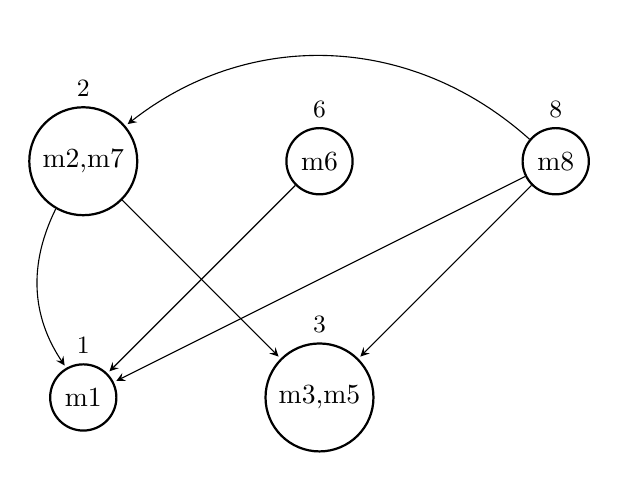
\begin{tikzpicture}%
		[>=stealth,
		shorten >=1pt,
		node distance=3cm,
		on grid,
		auto,
		every state/.style={draw=black!60, fill=black!5, very thick}
		]
		\tikzstyle{v}=[circle, minimum size=1mm,draw,thick]
		\node[v, label=above: {\small 1}] (n1) {m1};
		\node[v, label=above: {\small 2}] (n2)[above=of n1] {m2,m7};
		\node[v, label=above: {\small 3}] (n3)[right=of n1] {m3,m5};
		\node[v, label=above: {\small 6}] (n6)[right=of n2] {m6};
		\node[v, label=above: {\small 8}] (n8)[right=of n6] {m8};
		
		\path[->]
%		%   FROM  BEND/LOOP  POSITION OF LABEL   LABEL   TO
		(n8) edge (n1)
		(n8) edge[bend right=40] (n2)
		(n8) edge (n3)
		(n2) edge (n3)
		(n2) edge[bend right=30] (n1)
		(n6) edge (n1)
		;
		\end{tikzpicture}
	\end{center}
	\caption[Grafo de subsunci\'on para la Tabla~\ref{tables.examples.subsumptionEquivAndKilled}]{Grafo de \emph{Dynamic Mutant Subsumption} generado mediante la informaci\'on de la Tabla \ref{tables.examples.subsumptionEquivAndKilled}}
	\label{figures.examples.dynamicSubsumptionGraph}
\end{figure}

\subsection{Dynamic Mutant Subsumption como m\'etrica}
\label{sec:preliminares.mutation.whysubsumption}

En la secci\'on anterior presentamos las propiedades deseables en los mutantes generados por un operador de mutaci\'on, y algunas formas de evaluar el grado en que \'estas se cumplen. Sin embargo, al evaluar operadores de mutaci\'on con respecto a otros, o t\'ecnicas de selecci\'on de mutantes, la utilizaci\'on de m\'etricas como diferencia entre mutation score, cantidad de mutantes equivalentes generados (o evitados), ``dureza'' de mutantes (cuantos tests logra sobrevivir el mutante antes de ser detectado) y cantidad de mutantes, son las m\'as utilizadas.

En esta tesis se plantea utilizar \emph{Dynamic Mutant Subsumption} como una de las m\'etricas principales para evaluar a \emph{PRVO} con respecto al conjunto de operadores suficientes implementados en \emph{$\mu$Java}. La raz\'on de esto se debe a la cantidad de informaci\'on que permanece oculta al utilizar m\'etricas usuales.

Para utilizar un caso particular sobre el cual discutir las desventajas de las m\'etricas usuales vamos a referirnos a un trabajo publicado sobre un operador de mutaci\'on para fortalecer y debilitar expresiones booleanas (\textbf{B}oolean \textbf{E}xpression \textbf{E}xtender) \cite{bibliography.mutation.operators.beeBridaS17}. \'Este surge de la intuici\'on de que los operadores que afectan expresiones booleanas al modificar operadores (\emph{ROR}, \emph{COR}, \emph{COI}, entre otros) o reemplazar partes de la expresi\'on, como el caso de \emph{ROR} que reemplaza una expresi\'on boolena por las constantes \lstinline{True} y \lstinline{False}, generan cambios ``muy gruesos'' como cambiar una condici\'on de \textbf{a > b} por \textbf{a < b}, mientras que una modificaci\'on del estilo \textbf{a > b \&\& c} nos parece que puede llevar a mutantes m\'as sutiles. En este estudio utilizamos el mismos conjunto de operadores contra los que comparamos \emph{PRVO}, y evaluamos como la utilizaci\'on de \emph{BEE} afectaba a las siguientes m\'etricas:
\begin{description}[leftmargin=8em,style=nextline]
	\item[Mutation score] El decremento en el valor obtenido de mutation score al utilizar a \emph{BEE} servir\'ia como indicador de que mutantes m\'as dif\'iciles de detectar fueron generados. Mientras que un incremento indicar\'ia el aumento de mutantes m\'as triviales de detectar.
	\item[Cantidad de mutantes] Dado que en el peor caso es necesario ejecutar todos los tests para cada mutante (suponiendo un an\'alisis solo centrado en mutation score) los recursos utilizados por mutation testing, entre ellos tiempo, est\'an directamente relacionados a la cantidad de mutantes generados, todo operador deber\'ia ser evaluado con respecto al costo asociado, es decir, cuantos mutantes agrega al an\'alisis.
	\item[Dureza (toughness)] La cantidad de tests que un mutante es capaz de ``sobrevivir'', no ser detectado por, puede servir como una m\'etrica para evaluar cuan dif\'icil de detectar resulta. Analizar como cambia la dureza promedio de los mutantes detectados al agregar un operador (en este caso \emph{BEE}) permite evaluar la dificultad de detecci\'on de los mutantes agregados por el mismo.
	\item[Mutantes equivalentes] Una caracter\'istica negativa de un operador es cuantos mutantes equivalentes produce, \'estos son mutantes que si bien son distintos sint\'acticamente, son sem\'anticamente equivalentes al programa original, y por lo tanto imposibles de detectar.
	\item[Mutantes dif\'iciles de matar (stubborn)] La generaci\'on de mutantes dif\'iciles de matar (stubborn) es una caracter\'istica altamente deseable para un operador de mutaci\'on. Sin embargo representa una propiedad muy compleja para analizar, principalmente por la dificultad en dar una definici\'on apropiada, una de \'estas corresponde a la propuesta por Xiangjuan Yao et al. \cite{bibliography.mutation.evaluation.stubborn}: un mutante dif\'icil de matar es aquel para el cual existe un tests que es capaz de detectarlo pero no est\'a presente en una test suite ``suficientemente bueno'' la cual luego define como una test suite con 100\% de cobertura de ramas. Aunque finalmente se utilizan definiciones m\'as relajadas como la utilizaci\'on de testing exhaustivo acotado (considerar todas las entradas dentro de ciertas cotas) o generaci\'on de test suites mediante herramientas como \emph{EvoSuite} con una cobertura de ramas por encima del 80\%.
\end{description}

La evaluaci\'on presentada en \cite{bibliography.mutation.operators.beeBridaS17} utiliza estas m\'etricas para la evaluaci\'on del nuevo operador, y si bien los resultados no fueron negativos, \'estos no parecen mostrar una clara ventaja de utilizar el operador, aunque la motivaci\'on detr\'as del mismo as\'i como su definici\'on, parecer\'ia indiciar que el mismo tiene potencial. Un problema que tienen estos resultados es la cantidad de informaci\'on que permanece oculta. Como mencionamos en la secci\'on \ref{sec:preliminares.mutation.opevaluation}, el valor de mutation score se ve altamente afectado por: mutantes equivalentes, que disminuyen el valor sin significar una baja calidad de parte de los tests; mutantes triviales, que aumentan el valor mediante mutaciones que son triviales de detectar y no resultan en una evaluaci\'on apropiada de los tests; acoplamiento entre mutantes, cuando la detecci\'on de una mutaci\'on implica la detecci\'on de otra o cuando dos mutantes son equivalentes entre s\'i incrementan el mutation score por (en cierto modo) mutantes repetidos y lo mismo puede causar un decremento repetido en este valor.

El an\'alisis de mutantes equivalentes es un problema indecidible, an\'alisis manuales siguen siendo uno de los enfoques m\'as utilizados aunque sigue siendo una propiedad com\'unmente evaluada y con una gran importancia en comparaci\'on de operadores de mutaci\'on o t\'ecnicas de selecci\'on de mutantes.

La dificultad de detecci\'on de un mutante por el otro lado, es una propiedad que si bien ser\'ia interesante evaluar, resulta muy dif\'icil de definir, Visser presenta en \cite{bibliography.mutation.evaluation.hardnessVisser} un estudio sobre la dificultad de detectar mutantes el cual utiliza \emph{model counting} para evaluar la cantidad de escenarios (de manera exhaustiva, en un conjunto acotado) que logran diferenciar a un mutante del programa original. Este enfoque no resulta pr\'actico, algo que es mencionado en el trabajo anterior, y solo es posible en programas muy simples.

El uso de \emph{Dynamic Mutant Subsumption} a sido utilizado previamente para minimizar conjuntos de mutantes en \cite{bibliography.mutation.minimizing.dynamicsubsumption} y para medir la efectividad de un conjunto de mutantes en \cite{bibliography.mutation.efectiveness.dynamicsubsumption}, este \'ultimo trabajo sugiere la utilizaci\'on de dynamic mutant subsumption como forma de comparar operadores de mutaci\'on y/o t\'ecnicas de selecci\'on de mutantes. Una ventaja inicial de utilizar esta t\'ecnica es que la definici\'on es clara, un mutante subsume a otro si ambos son detectados y los tests que detectan al primero tambi\'en detectan al segundo. A su vez, la conclusi\'on de que los mutantes subsumidos son redundantes se relaciona a la existencia de otro/s mutantes que ejercitan al conjunto de tests de manera m\'as espec\'ifica (son detectados por menos tests), y los mutantes equivalentes con respecto a subsunci\'on ejercitan varias veces al mismo conjunto de tests, pudiendo elegir un solo representante de \'estos. La dificultad de detecci\'on puede asociarse a subsunci\'on argumentando que si un mutante subsume a otros, es detectado por menos tests, dando la intuici\'on de que requiere tests m\'as espec\'ificos que los mutantes que subsume.

Retomando el estudio sobre el operador \emph{BEE}, cuando realizamos un an\'alisis de subsunci\'on logramos obtener resultados mas significativos con respecto a la utilidad del operador para mutation testing. Las preguntas de investigaci\'on de este trabajo son:
\begin{quote}
	{\it Nuestro operador (BEE) genera mayor cantidad de mutantes dif\'iciles de matar (stubborn) que los operados existentes que debilitan o fortalecen expresiones booleanas?}
\end{quote}
\begin{quote}
	{\it Como nuestro operador (BEE) afecta al an\'alisis de mutaci\'on?}
\end{quote}

Siendo los resultados obtenidos los de las Tablas \ref{tables.examples.bee.paperResults.arraypartition}, \ref{tables.examples.bee.paperResults.binaryheap}, \ref{tables.examples.bee.paperResults.ordset}, \ref{tables.examples.bee.paperResults.treemap}, y \ref{tables.examples.bee.paperResults.trityp}. Estos resultados dieron lugar a la conclusi\'on de que la respuesta a la primer pregunta de investigaci\'on es negativa (\emph{BEE} no parece generar una cantidad importante de mutantes dif\'iciles de matar), mientras que la segunda pregunta se responde de una manera m\'as positiva al indicar que la dificultad de matar los mutantes generados por \emph{BEE} parece mantenerse con respecto al resto de los mutantes (el valor de \emph{toughness} pr\'acticamente no cambia) y que la cantidad de mutantes equivalentes generados se deben a particularidades de algunos casos. Un problema con los resultados utilizados es que parecen estar ocultando informaci\'on. Por esto, al realizar un an\'alisis de los mismos casos utilizados en el trabajo publicado, pero utilizando Dynamic Mutant Subsumption, obtenemos los resultados en la Figura~\ref{subsumption-results-bee} que permiten observar que en tres de los cinco casos de estudio (\emph{BinaryHeap}, \emph{OrdSet}, y \emph{TreeMap}) los mutantes generados por \emph{BEE} son dominadores, es decir, corresponden a mutantes no redundantes para evaluar a los tests. En los casos de \emph{BinaryHeap} y \emph{OrdSet} se observa que al menos el 50\% de los mutantes dominadores generador por \emph{BEE} no son equivalentes a otros mutantes dominadores, lo que permite concluir que representan fallas nuevas no generadas por los otros operadores.

Esta comparaci\'on sirve de argumento para utilizar Dynamic Mutant Subsumption como una de las principales t\'ecnicas para evaluar un operador de mutaci\'on.

\begin{table}[]
	\caption[Resultados de la evaluaci\'on de \emph{BEE} para \emph{ArrayPartition}]{Datos de evaluaci\'on de \emph{BEE} para \emph{ArrayPartition} de acuerdo al trabajo presentado en \cite{bibliography.mutation.operators.beeBridaS17}}
	\label{tables.examples.bee.paperResults.arraypartition}
	\centering
	\scriptsize
	\def\arraystretch{0.95}
	\setlength\tabcolsep{0.5mm}
	\begin{tabular}{c|ccccc|}
		\cline{2-6}
		& Mutantes & Sobrevivientes & Toughness (killed) & Mutation score & Stubborn \\ \hline
		\multicolumn{1}{|c|}{SIN BEE} & 196 & 14 & 0.50 & 92.85\% & 6 \\ \hline
		\multicolumn{1}{|c|}{CON BEE} & 336 & 36 & 0.53 & 89.28\% & 8 \\ \hline
	\end{tabular}
\end{table}

\begin{table}[]
	\caption[Resultados de la evaluaci\'on de \emph{BEE} para \emph{BinaryHeap}]{Datos de evaluaci\'on de \emph{BEE} para \emph{BinaryHeap} de acuerdo al trabajo presentado en \cite{bibliography.mutation.operators.beeBridaS17}}
	\label{tables.examples.bee.paperResults.binaryheap}
	\centering
	\scriptsize
	\def\arraystretch{0.95}
	\setlength\tabcolsep{0.5mm}
	\begin{tabular}{c|ccccc|}
		\cline{2-6}
		& Mutantes & Sobrevivientes & Toughness (killed) & Mutation score & Stubborn \\ \hline
		\multicolumn{1}{|c|}{SIN BEE} & 454 & 111 & 0.73 & 75.55\% & 65 \\ \hline
		\multicolumn{1}{|c|}{CON BEE} & 889 & 341 & 0.72 & 61.64\% & 163 \\ \hline
	\end{tabular}
\end{table}

\begin{table}[]
	\caption[Resultados de la evaluaci\'on de \emph{BEE} para \emph{OrdSet}]{Datos de evaluaci\'on de \emph{BEE} para \emph{OrdSet} de acuerdo al trabajo presentado en \cite{bibliography.mutation.operators.beeBridaS17}}
	\label{tables.examples.bee.paperResults.ordset}
	\centering
	\scriptsize
	\def\arraystretch{0.95}
	\setlength\tabcolsep{0.5mm}
	\begin{tabular}{c|ccccc|}
		\cline{2-6}
		& Mutantes & Sobrevivientes & Toughness (killed) & Mutation score & Stubborn \\ \hline
		\multicolumn{1}{|c|}{SIN BEE} & 1278 & 179 & 0.83 & 85.99\% & 160 \\ \hline
		\multicolumn{1}{|c|}{CON BEE} & 2248 & 620 & 0.83 & 72.41\% & 403 \\ \hline
	\end{tabular}
\end{table}

\begin{table}[]
	\caption[Resultados de la evaluaci\'on de \emph{BEE} para \emph{TreeMap}]{Datos de evaluaci\'on de \emph{BEE} para \emph{TreeMap} de acuerdo al trabajo presentado en \cite{bibliography.mutation.operators.beeBridaS17}}
	\label{tables.examples.bee.paperResults.treemap}
	\centering
	\scriptsize
	\def\arraystretch{0.95}
	\setlength\tabcolsep{0.5mm}
	\begin{tabular}{c|ccccc|}
		\cline{2-6}
		& Mutantes & Sobrevivientes & Toughness (killed) & Mutation score & Stubborn \\ \hline
		\multicolumn{1}{|c|}{SIN BEE} & 576 & 160 & 0.93 & 72.22\% & 114 \\ \hline
		\multicolumn{1}{|c|}{CON BEE} & 2536 & 1376 & 0.94 & 45.74\% & 631 \\ \hline
	\end{tabular}
\end{table}

\begin{table}[]
	\caption[Resultados de la evaluaci\'on de \emph{BEE} para \emph{TriTyp}]{Datos de evaluaci\'on de \emph{BEE} para \emph{TriTyp} de acuerdo al trabajo presentado en \cite{bibliography.mutation.operators.beeBridaS17}}
	\label{tables.examples.bee.paperResults.trityp}
	\centering
	\scriptsize
	\def\arraystretch{0.95}
	\setlength\tabcolsep{0.5mm}
	\begin{tabular}{c|ccccc|}
		\cline{2-6}
		& Mutantes & Sobrevivientes & Toughness (killed) & Mutation score & Stubborn \\ \hline
		\multicolumn{1}{|c|}{SIN BEE} & 435 & 109 & 0.98 & 74.94\% & 56 \\ \hline
		\multicolumn{1}{|c|}{CON BEE} & 55 & 115 & 0.98 & 79.27\% & 62 \\ \hline
	\end{tabular}
\end{table}

\begin{figure}[t]
	\begin{center}
		\includegraphics[width=12cm]{figures/BEETables.png}
	\end{center}
	\caption{Dynamic subsumption analysis para el operador \emph{BEE}}
	\label{subsumption-results-bee}
\end{figure}